We discuss the performance of the centralized algorithms in Section \ref{sec-3} for some system configurations. To begin with, we consider a single cell \ac{SISO} model operating at \me{10} dB \ac{SNR} with \me{K = 3} users sharing \me{N = 3} sub-channel resources. The total number of backlogged packets waiting at the transmitter for each user is given by \me{Q_1 = 4}, \eqn{Q_2 = 8} and \me{Q_3 = 4} bits, respectively. 
\begin{table}
	\centering
	\caption{Number of backlogged bits associated with each user for a system \me{\lbrace N,N_B,K,N_R \rbrace = \lbrace 5,2,8,1 \rbrace}.}
	\renewcommand{\arraystretch}{1.25} \scriptsize
	\begin{tabular}{|c|*{8}{c}|c|}
		\hline
		\multirow{2}{*}{\me{q}} & \multicolumn{8}{c|}{user indices} & \multirow{2}{*}{\me{\chi}} \\
		\cline{2-9}
		& 1 & 2 & 3 & 4 & 5 & 6 & 7 & 8 & \\
		\hline
		\hline
		\me{1} & 15.0 & 3.95 & 5.26 & 8.95 & 7.0 & 11.9 & 12.0 & 9.7 & 25.15 \\
		\me{2} & 11.2 & 3.9 & 10.76 & 10.65 & 10.27 & 9.68 & 8.77 & 5.9 & 27.77 \\
		\me{\infty} & 11.4 & 4.4 & 10.4 & 10.4 & 10.4 & 8.4 &  8.4 &  6.4 & 28.68 \\
		\hline
		\me{Q_k}  & 15.0 &  8.0 &  14.0 & 14.0 &  14.0 & 12.0 & 12.0 & 10.0  \\
		\cline{1-9}
	\end{tabular}
	\label{tbl-3}
\end{table}

Table \ref{tbl-1} tabulates the channels of the users over each sub-channel followed by the rates assigned by three different algorithms, \ac{Q-WSRME} allocation, \ac{JSFRA} approach and the sub-channel wise \ac{Q-WSRM} scheme using the \ac{MSE} reformulation for all cases \cite{christensen2008weighted}. The metric used for the comparison is the total number of backlogged bits left over after each transmission, which is denoted as \me{\chi = \sum_{k = 1}^K \; [ Q_k - t_k ]^+}. Even though \me{\mc{U}(1)} and \me{\mc{U}(3)} have equal number of backlogged packets of \me{Q_{1} = Q_{3} = 4} bits, user \me{\mc{U}(3)} is scheduled in the first sub-channel due to the better channel condition. In contrast, the \ac{JSFRA} approach assigns the first user on the first sub-channel, which reduces the total number of backlogged packets. The rate allocated for \me{\mc{U}(2)} on the second sub-channel is higher in \ac{JSFRA} scheme compared to the others. It is due to the efficient allocation of the total power shared across the sub-channels.

For a \ac{MIMO} setup, we consider a system with \me{N=4} and \eqn{N=2} sub-channels with \me{N_B = 3} \acp{BS}, each equipped with \me{N_T = 4} transmit antennas operating at \me{10}dB \ac{SNR}, serving \me{|\mc{U}_b| = 3} users each. The \ac{PL} difference between the \acp{BS} and the users are uniformly generated from \me{[0,-3]} dB and the \ac{BS}-user associations are made by selecting the \ac{BS} with the lowest \ac{PL} component. Fig. \subref*{fig-1} and Fig. \subref*{fig-2} compares the performance of the centralized schemes for \eqn{N_R = 1} and \me{N_R = 2} receive antenna cases respectively.
%The total number of queued packets for Fig. \subref*{fig-1} is given by \me{Q_k = [14,15,14,8,12,9,12,11,11]} bits and for Fig. \subref*{fig-2} is \me{Q_k = [9,12,8,12,5,4,10,8,5]} bits respectively.
\begin{figure}
	\centering
	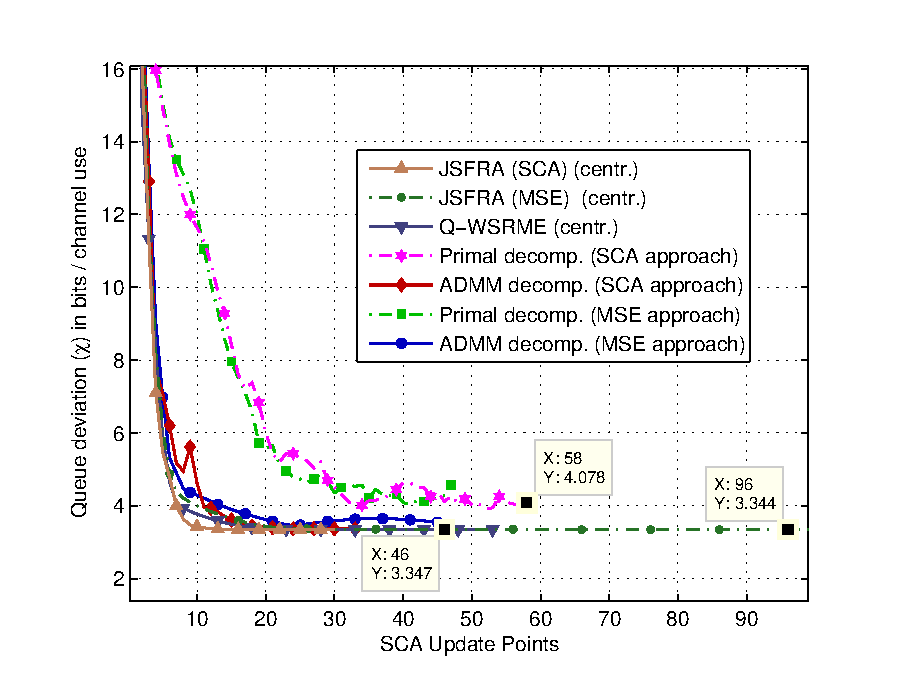
\includegraphics[width=\columnwidth]{fig-3-2}
	\vspace{-0.3in}
	\caption{Convergence of the centralized and the distributed algorithms for \me{\lbrace N,N_B,K,N_T,N_R \rbrace = \lbrace 3,2,8,4,1 \rbrace} using \me{\ell_1} norm for \ac{JSFRA} schemes with \me{Q_k = [5,7,9,11,8,12,5,4]} bits}
	\label{fig-d}
\end{figure}

The comparison in Fig. \ref{fig-a} is made in terms of the total number of residual bits remaining in the system after each \ac{SCA} update. The \ac{Q-WSRM} scheme is not optimal due to the problem of over-allocation when the number of queued packets is small. In contrast, the \ac{Q-WSRME} algorithm provides better allocation with the explicit rate constraint to avoid the over-allocation. For both scenarios in Fig. \ref{fig-a}, the \ac{Q-WSRME} performs marginally inferior to the \ac{JSFRA} algorithms due to the weights used in the algorithm, since the \ac{Q-WSRME} scheme favors the users with the large number of backlogged packets as compared to the users with better channel conditions. Note that the receivers are updated along with the \ac{SCA} update instants \textit{i.e}, \me{K_{\max} = 1} for both Fig. \subref*{fig-1} and Fig. \subref*{fig-2}. However, the performance loss incurred by the combined update of the \ac{SCA} operating point and the receiver is marginal.

The behavior of the \ac{JSFRA} algorithm for different exponents \me{q} is outlined in the Table \ref{tbl-3} for the users located at the cell-edge of the system employing \me{N_T = 4} transmit antennas. It is evident that the \ac{JSFRA} algorithm minimizes the total number of queued bits for the \me{\ell_1} norm compared to the \me{\ell_2} norm, which is shown in the column displaying the total number of left over packets \me{\chi} in bits. The \me{\ell_{\infty}} norm provides fair allocation of the resources by making the leftover packets to be equal for all users to \me{\chi_k = 3.58} bits.
